\chapter{Implementation}
\label{ch:implementation}

\section{Fabric SDK}
\label{sec:implementation:sdk}
The Hyperledger Fabric Client SDK provides APIs to interact with the Hyperledger Fabric blockchain, for instance, provides APIs to interact with smart contracts, submit transactions to a ledger, and query the ledger \cite{fabric-sdk-node}. The Fabric SDK provides the following packages:
\begin{itemize}
    \item \lstinline{fabric-ca-client} - The fabric-ca provides APIs to register and to enroll participants(admin/patient/doctor) to establish trusted identities on the blockchain network. The package creates a new CA client for interacting with the CA server of the hospital to register and enroll the participants. 
    \item \lstinline{fabric-common} - encapsulates the common code used by all fabric-sdk-node packages supporting fine-grain interactions with the Fabric network to send transaction invocations. Provides APIs to monitoring events, logging and configuration settings of the environment variable, program arguments, in-memory settings
    \item \lstinline{fabric-network} - This package contains the APIs required to connect to the Fabric network, submit transactions to query or edit  the ledger. Provides APIs to manage the wallet which is used for managing identities and create a connection profile based on the \href{https://github.com/kshitijyelpale/blockchain-hyperledger-fabric-electronic-patient-records/blob/main/app/first-network/organizations/ccp-template.json}{connection profile JSON} generated when CA is created.
\end{itemize}
In package fabric-network - The main class that allows the Fabric SDK to interact with the network is the Gateway class. Once instantiated, the object create a gateway/connection to a peer/user within the blockchain network and enables access to the chaincode and channels for which that peer/user is a member.  \cite{fabric-sdk-node}.



%
% Section: Steps to use the application 
%
\section{Steps to use the application}
\label{sec:implementation:steps}
This section describes very detailed steps to run the application start from the prerequisites. The project is available on \href{https://github.com/kshitijyelpale/blockchain-hyperledger-fabric-electronic-patient-records}{GitHub} 

\subsection{Prerequisites}
The system should have installed some tools such as docker, docker-compose, node, npm, golang, curl. Follow the detailed steps on the official website of fabric for the specific version and commands \cite{prerequisites}.

Download the fabric basic framework which generates platform-specific binaries and Docker images \cite{download-fabric-samples}.
Execute the following curl command.

\lstinline{curl -sSL https://bit.ly/2ysbOFE | bash -s -- 2.2.2 1.4.9}

This generates all test network code in folder 'fabric samples'. Now clone this project's git repository. Copy bin directory from 'fabric samples' to
\lstinline{blockchain-hyperledger-fabric-electronic-patient-records/app}.

\subsection{Start network}
\label{sec:implementation:steps:startnetwork}

Go to the first network directory and execute the network.sh file with argument up. 

\lstinline{./network up} 

This command brings up all docker containers required for two hospital organizations.

\lstinline{./network createChannel} 

This command creates a channel 'hospitalChannel' on which both organizations are connected.

\lstinline{./network deployCC} 

This command packages the smart contract code inside 'patient-asset-transfer'. The initial data of six patients are created in a ledger 
The folder structure looks similar to fabric samples which helps a developer who is already worked with the test network. 

\subsection{Add additional hospital}
\label{sec:implementation:steps:additionalhospital}

In addition to the existing two hospital organizations, one can also add a new hospital organization called hosp3. Go inside 'addHosp3' of the first-network directory.

\lstinline{./addHosp3 up}

This command brings up the containers required for hospital3 to work and join 'hospitalChannel'. If there are multiple channels in the network, it is mandatory to specify which channel to connect to. 

\lstinline{./addHosp3 deployCC} 

This command installs chaincode on hosp3 nodes. Hosp3 added separately to show that framework provides pluggable architecture. On scaling the network, new organizations can be easily added without down the existing network. Still, this solution is needed to be improved to support this pluggable feature more mature. Few things are hardcoded in the backend and front end.

\subsection{Bring up the backend and frontend}
\label{sec:implementation:steps:bringupbackend}

Go to app/server. 

\lstinline{npm install} 

This command installs all dependency files required for the backend server to run.

\lstinline{npm start} 

This command starts the express js backend server. It also enrolls and registers few users from the network. It includes both admin users from hospital organizations, initial six patient data, and four doctors. The users are created inside the wallet.  
Now go to app/client

\lstinline{npm install} 

\lstinline{ng serve -o} 

This brings up the angular server and automatically opened up in the default browser.   

%
% Section: Screenshots  
%
\section{Workflow} 
\label{sec:implementation:screenshots}

This section describes the working of the application through the perspective of all users - admin, patient, and doctor.

\subsection{Login Admin}
An admin is created for each hospital that joins the network. The details of the admin must be present during the addition of the hospital to the network. The admin details (username and password) are present in the fabric-ca-server-config.yaml of the respective hospital CA configuration. The login page for the admin is as shown in Figure \ref{fig:chapter03:admin1} the role admin has to be chosen, as the web application is the same for all the participants, the admin must choose the hospital and enter the credentials. These credentials are checked against the credentials stored in the blockchain network which was configured in the Hospital CA config YAML file.
\begin{figure}[htbp]
 \centering
 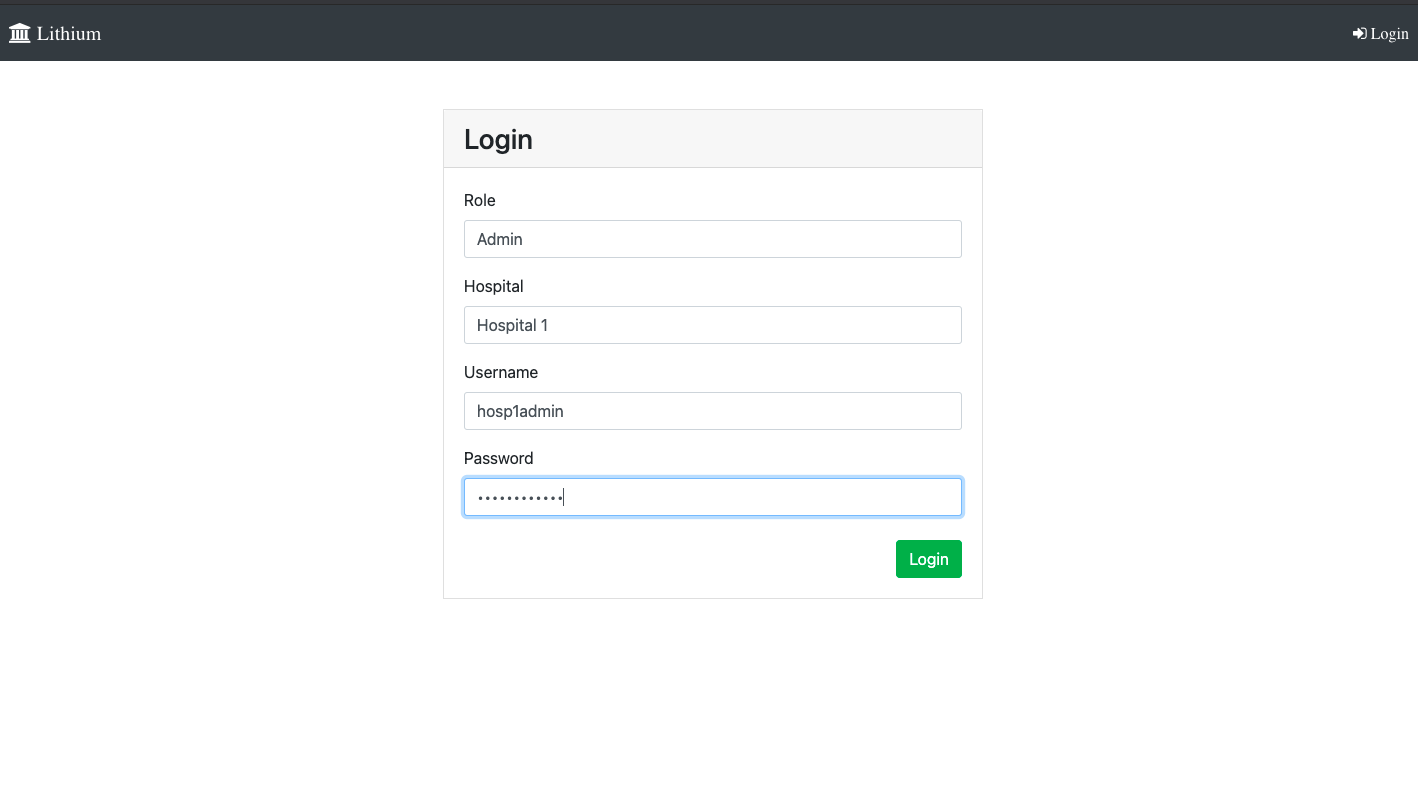
\includegraphics[height=8cm]{gfx/figures/admin1.png}
 \caption{Admin Loogin Screen}
 \label{fig:chapter03:admin1}
\end{figure}

\subsection{Admin Dashboard}
As soon the admin log in successfully, a dashboard is displayed which contains the list of all the patients in the network and the functions highlighted in Figure \ref{fig:chapter03:admin2}. The patient list is retrieved by invoking the admin contract through which a transaction is created in the ledger to retrieve all the patient objects in the world state. The admin has access only to the names of the patient other details are restricted by the contract.
\begin{figure}[htbp]
 \centering
 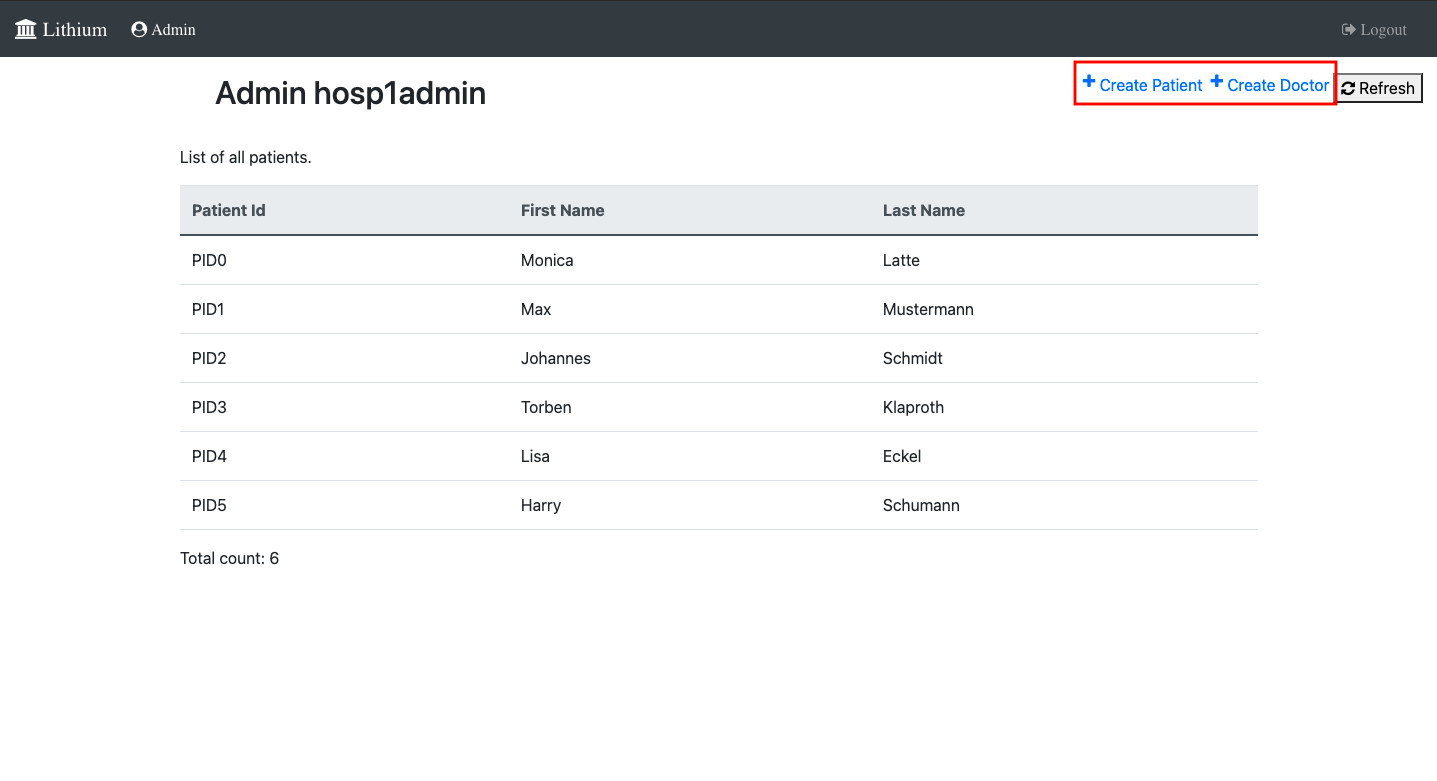
\includegraphics[height=8cm]{gfx/figures/admin2.png}
 \caption{Admin Dashboard}
 \label{fig:chapter03:admin2}
\end{figure}

\subsection{Create Patient}
The admin has the capability to create a patient that is creating a transaction in the ledger to create an object to the world state. The admin must enter the basic info of the patient as shown in Figure \ref{fig:chapter03:admin4} on save a transaction is created in the ledger and sent to all the peers of the network. The patient data is validated and if valid endorsed and stored in the ledger. The patient is also created as a client in the network using this client the patient can interact with the ledger. And on save, temporary patient credentials are created, which the patient must change on the first login for security reasons. Figure \ref{fig:chapter03:admin5} shows the list of all patients, the created patient was added to the ledger and hence is retrieved when all the patients are queried again.
\begin{figure}[htbp]
 \centering
 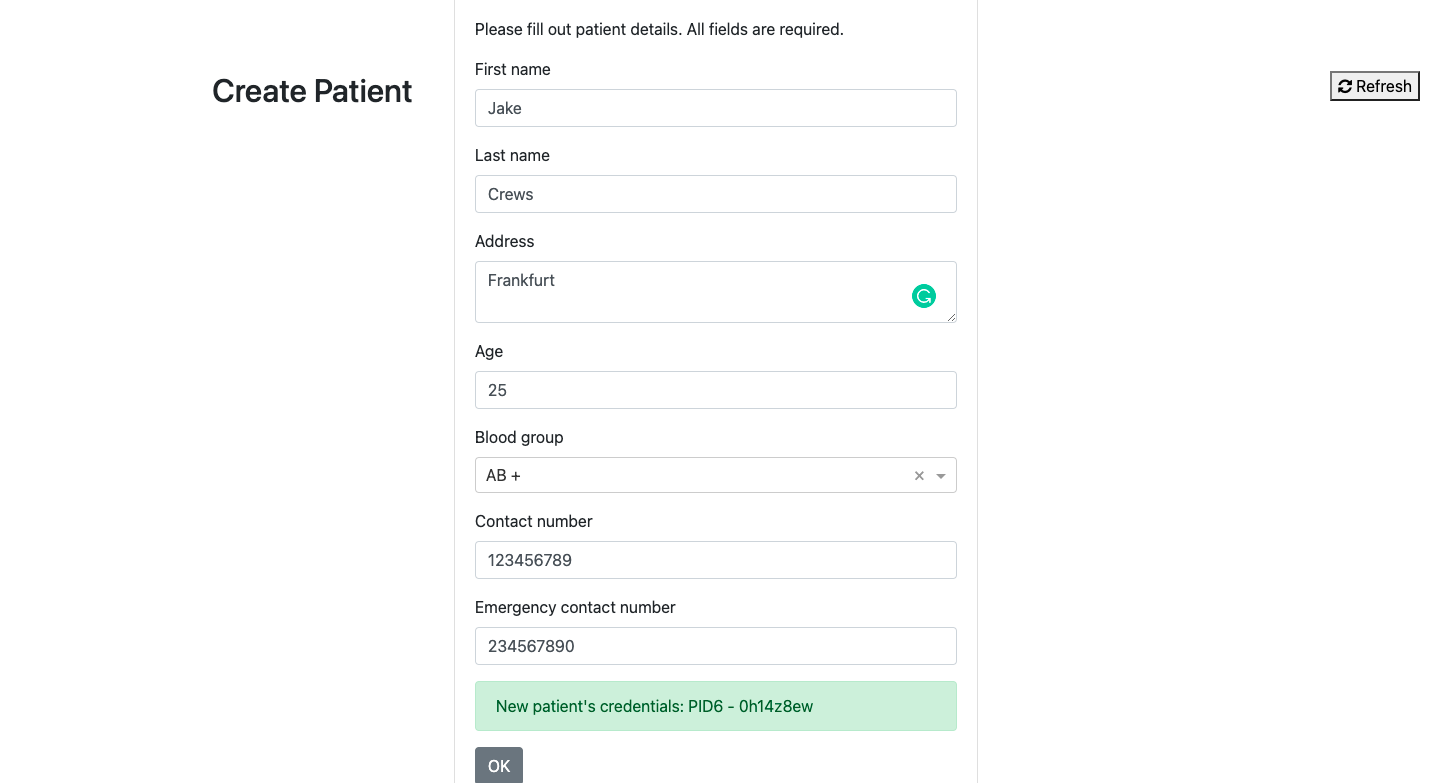
\includegraphics[height=8cm]{gfx/figures/admin4.png}
 \caption{Create Patient}
 \label{fig:chapter03:admin4}
\end{figure}
\begin{figure}[htbp]
 \centering
 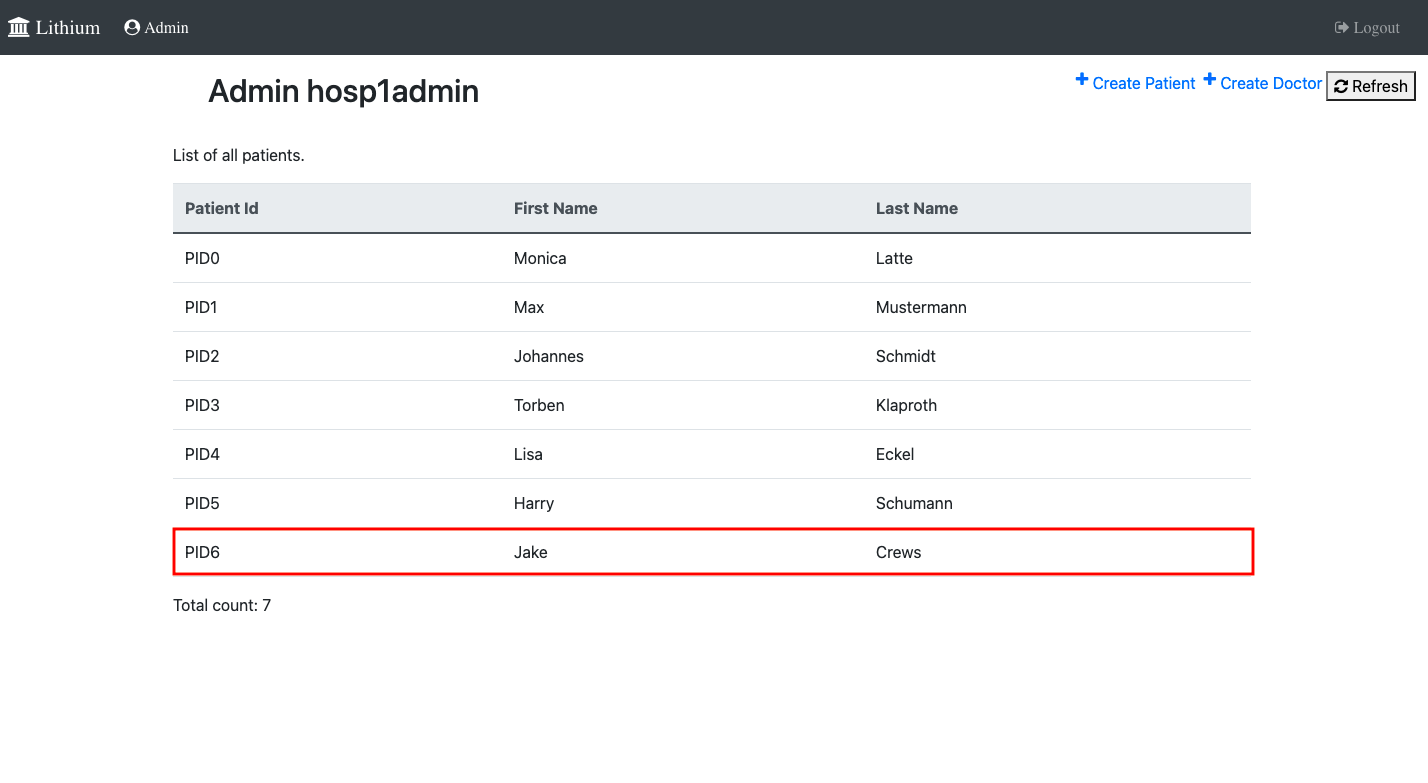
\includegraphics[height=8cm]{gfx/figures/admin5.png}
 \caption{Admin Dashboard}
 \label{fig:chapter03:admin5}
\end{figure}

\subsection{Create Doctor}
The admin can also create a doctor. As the doctor is not an object that is stored in the ledger, a client is created in the network using which the doctor now can interact with the ledger. There is no interaction with the ledger on the creation of the doctor. The admin must enter the details of the doctor as shown in Figure \ref{fig:chapter03:admin6} and on save a client is created in the network.
\begin{figure}[htbp]
 \centering
 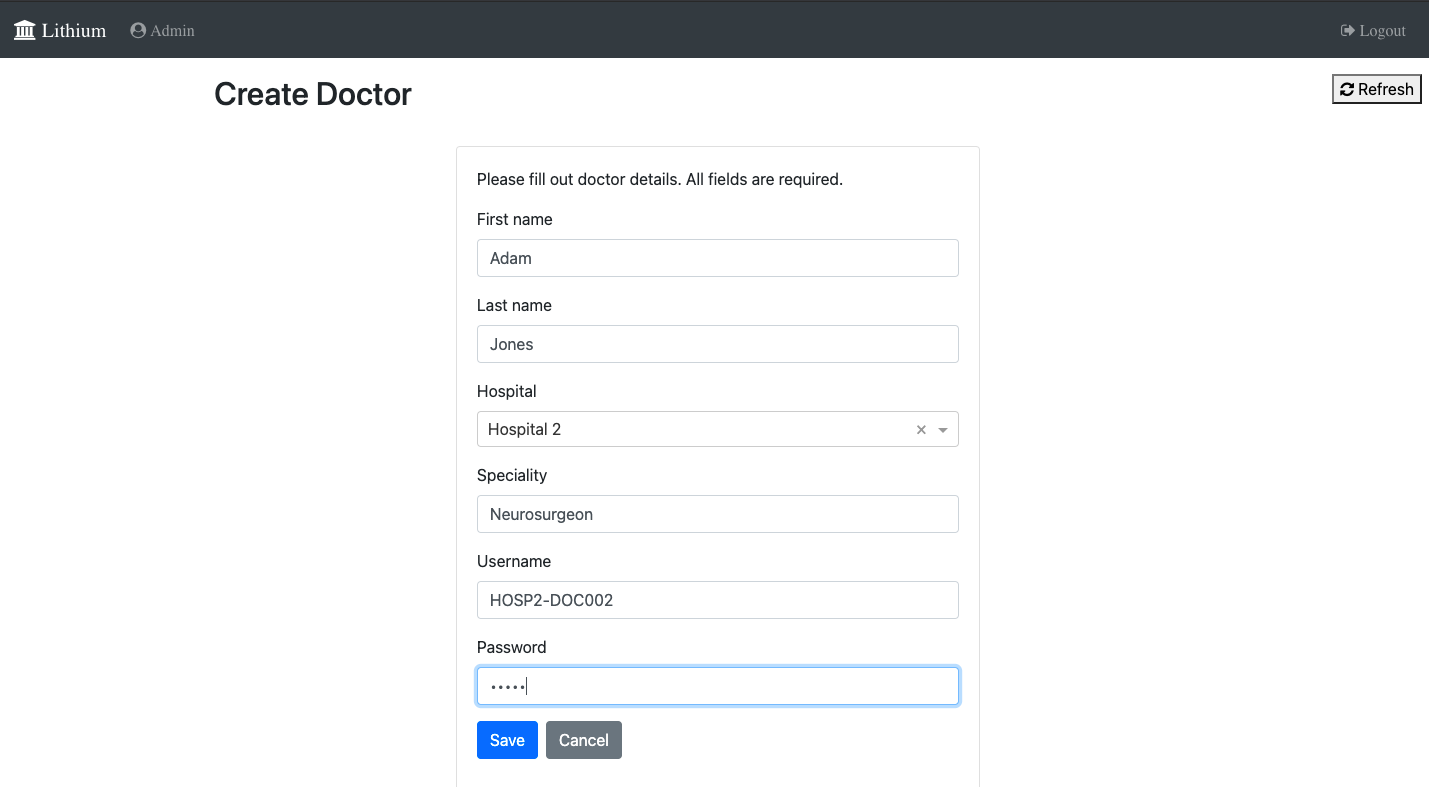
\includegraphics[height=8cm]{gfx/figures/admin6.png}
 \caption{Create Doctor}
 \label{fig:chapter03:admin6}
\end{figure}

\subsection{Login Patient}
The hospital provides patient his/her username and temporary password during the first visit to the hospital. If the patient is logging in for the first time, then after selecting role as patient and entering username and password provided by hospital, gets the message requesting to change the temporary password immediately as shown in Figure \ref{fig:chapter04:patient1}. The patient has to enter new password as per his/her choice as shown in Figure \ref{fig:chapter04:patient2}. The new password is then hashed and stored in ledger. So, from next time, whenever the patient wants to login, just has to select role, and enter username and new password. Both the temporary and new password are hashed and stored in the ledger. During every login, the entered password is hashed and compared with the hash value of password stored in ledger.
\begin{figure}[htbp]
 \centering
 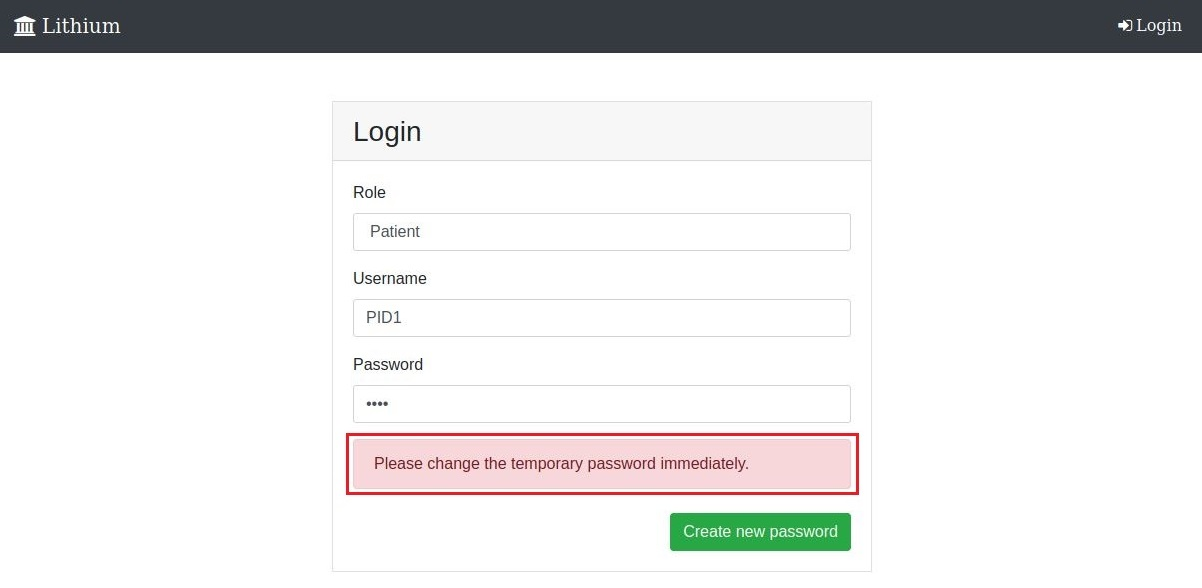
\includegraphics[width=1.1\textwidth, height=7.5cm]{gfx/figures/patient1.jpg}
 \caption{Login Patient}
 \label{fig:chapter04:patient1}
\end{figure}

\begin{figure}[htbp]
 \centering
 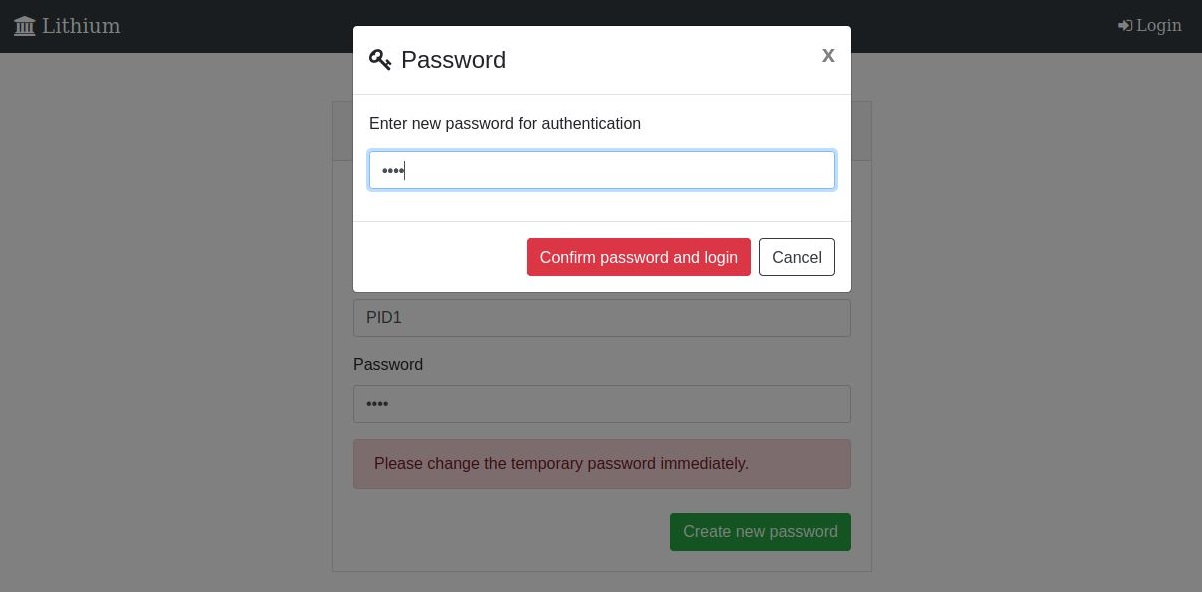
\includegraphics[width=1.1\textwidth, height=7.5cm]{gfx/figures/patient2.jpg}
 \caption{New Password}
 \label{fig:chapter04:patient2}
\end{figure}

\subsection{View Patient Details}
After successful login, the patient can view his/her personal as well as medical details as shown in Figure \ref{fig:chapter04:patient3}. The patient details are retrieved from the world state by invoking the patient contract.

\begin{figure}[htbp]
 \centering
 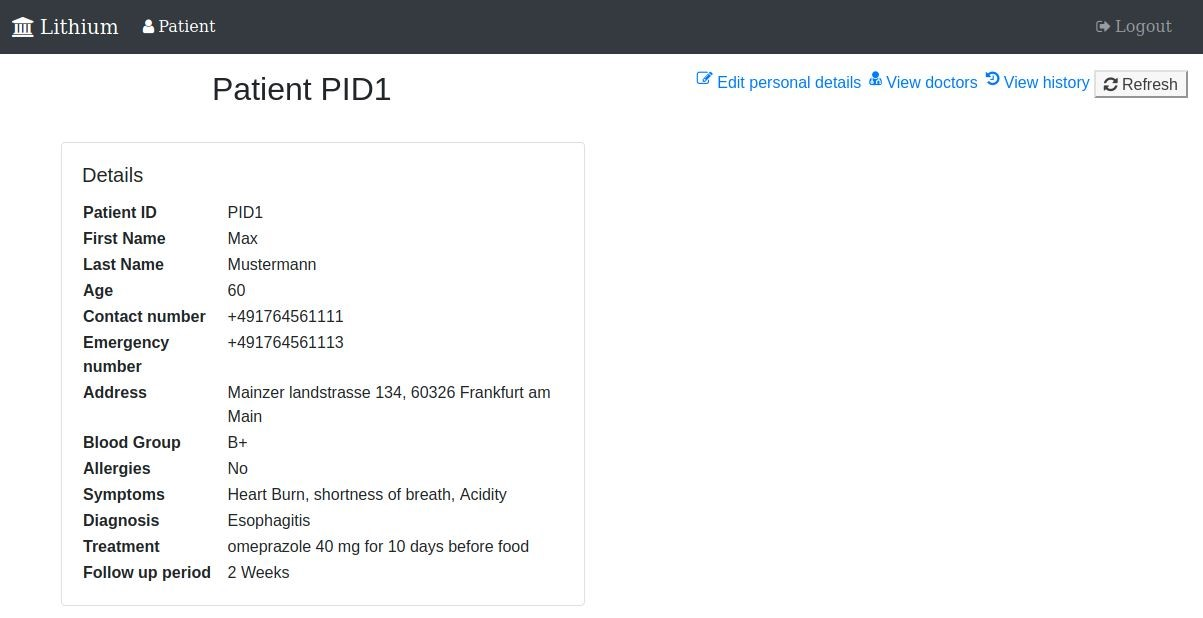
\includegraphics[width=1.1\textwidth, height=7cm]{gfx/figures/patient3.jpg}
 \caption{View Patient Details}
 \label{fig:chapter04:patient3}
\end{figure}

\subsection{Grant/Revoke Access}
On selecting \textit{View doctors}, it displays a list of doctors from both the hospitals  as shown in Figure \ref{fig:chapter04:patient4}. The patient has the right to grant or revoke the access to/from the doctor. When patient grants access to the doctor only then the doctor can view patient's medical details and medical history, When patient revokes the access, then doctor is unable to access patient's medical records, 

\begin{figure}[htbp]
 \centering
 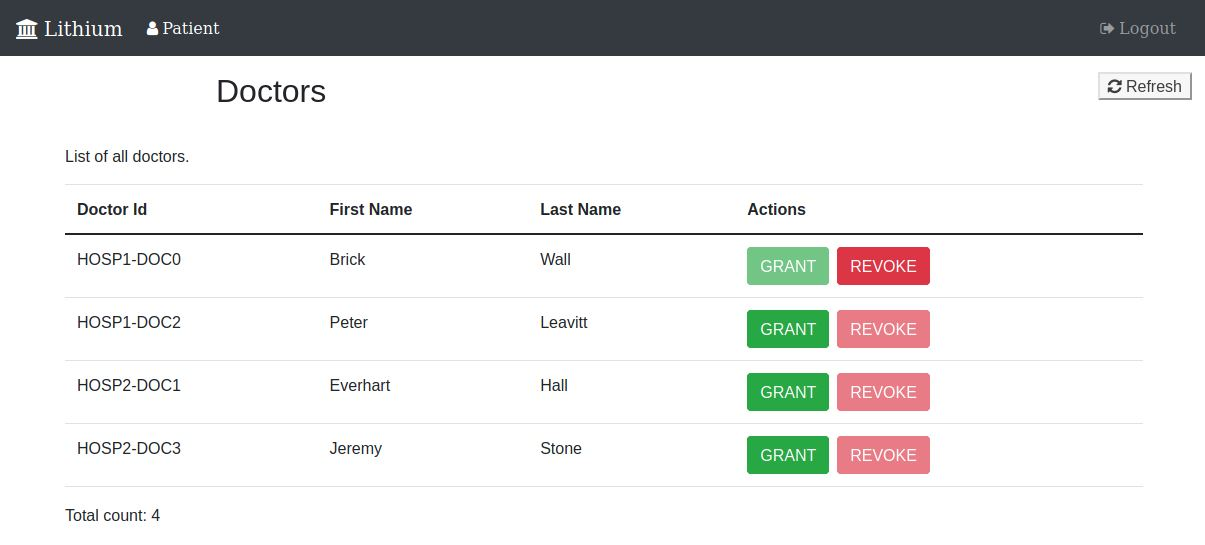
\includegraphics[width=1.1\textwidth, height=7cm]{gfx/figures/patient4.jpg}
 \caption{Grant/Revoke access}
 \label{fig:chapter04:patient4}
\end{figure}

\subsection{Edit Personal Details}
The patient can edit his/her personal details as shown in Figure \ref{fig:chapter04:patient5}. If any changes are made, then the new details are updated in the ledger using patient contract.

\begin{figure}[htbp]
 \centering
 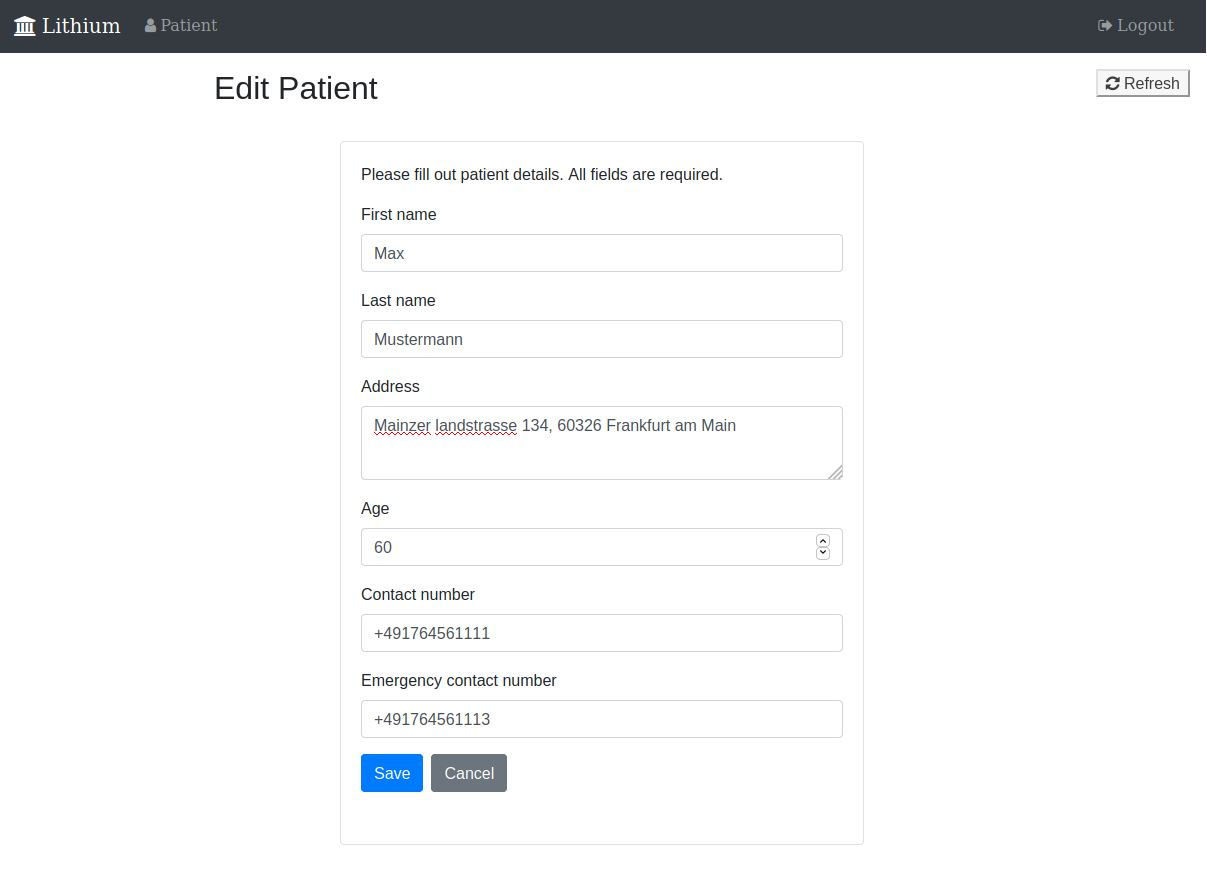
\includegraphics[width=1.1\textwidth, height=7cm]{gfx/figures/patient5.jpg}
 \caption{Edit personal details}
 \label{fig:chapter04:patient5}
\end{figure}

\subsection{View History}
The patient can view all the records, personal and medical starting from the first visit to the latest visit to all the doctors as shown in Figure \ref{fig:chapter04:patient5} . This functionality is possible because of the presence of getHistoryForKey API in hyperledger fabric which returns the history of the patient. This provides complete transparency of the transactions to the patient.

\begin{figure}[htbp]
 \centering
 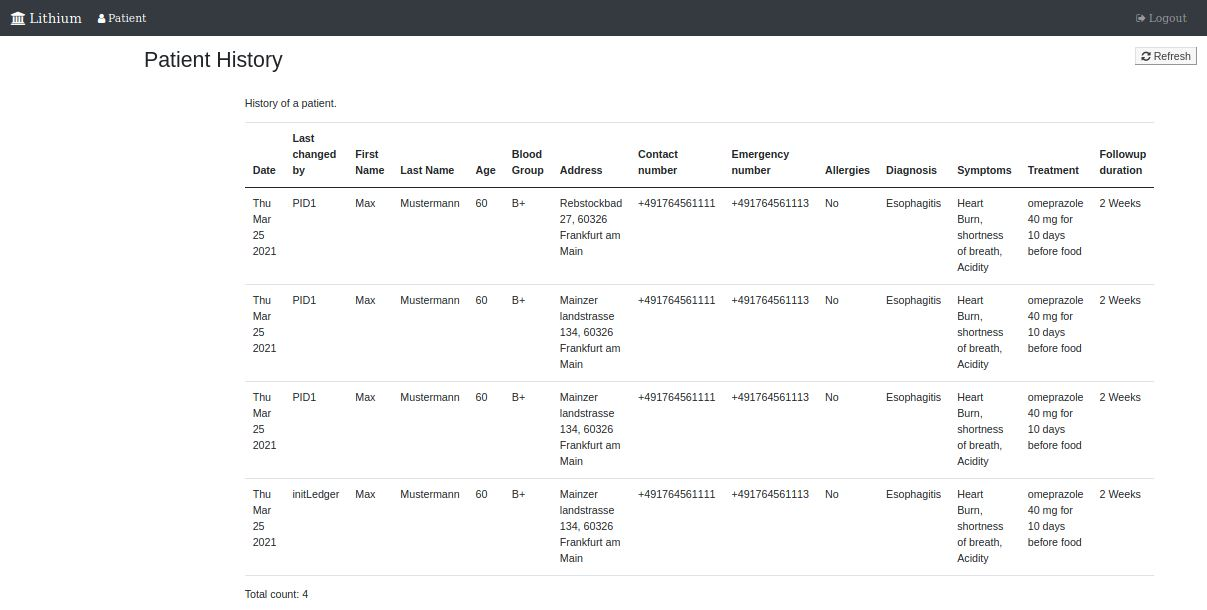
\includegraphics[width=1.1\textwidth, height=7cm]{gfx/figures/patient6.jpg}
 \caption{View patient's history}
 \label{fig:chapter04:patient6}
\end{figure}

\subsection{Login Doctor and View Doctor Details}
To login as doctor, user need to select 'Doctor' as a role, hospital which he/she belong and right credentials on login page as mentioned in the Figure \ref{fig:chapter04:doctor1}.

\begin{figure}[htbp]
 \centering
 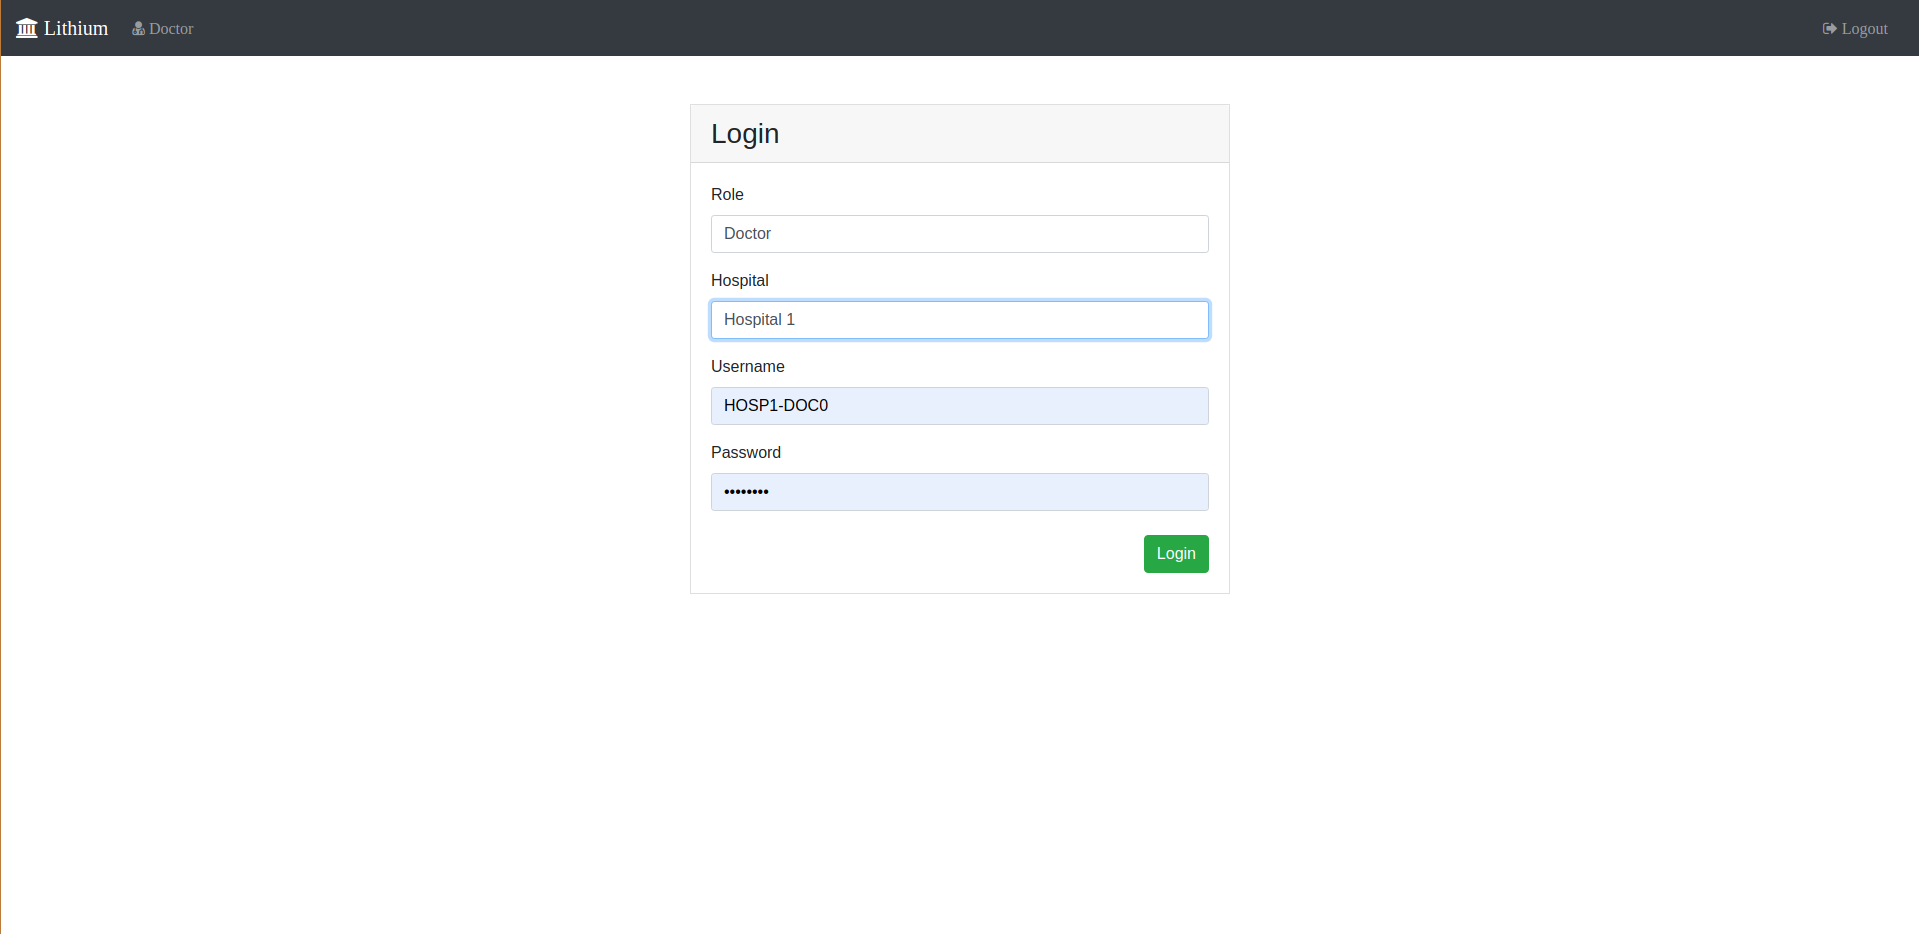
\includegraphics[width=1.1\textwidth, height=7cm]{gfx/figures/doctor1.png}
 \caption{Login Doctor}
 \label{fig:chapter04:doctor1}
\end{figure}

After successfully logged in as a doctor, the doctor details showed just like patient details. Here only few fields of the doctor shown in Figure \ref{fig:chapter04:doctor2}

\begin{figure}[htbp]
 \centering
 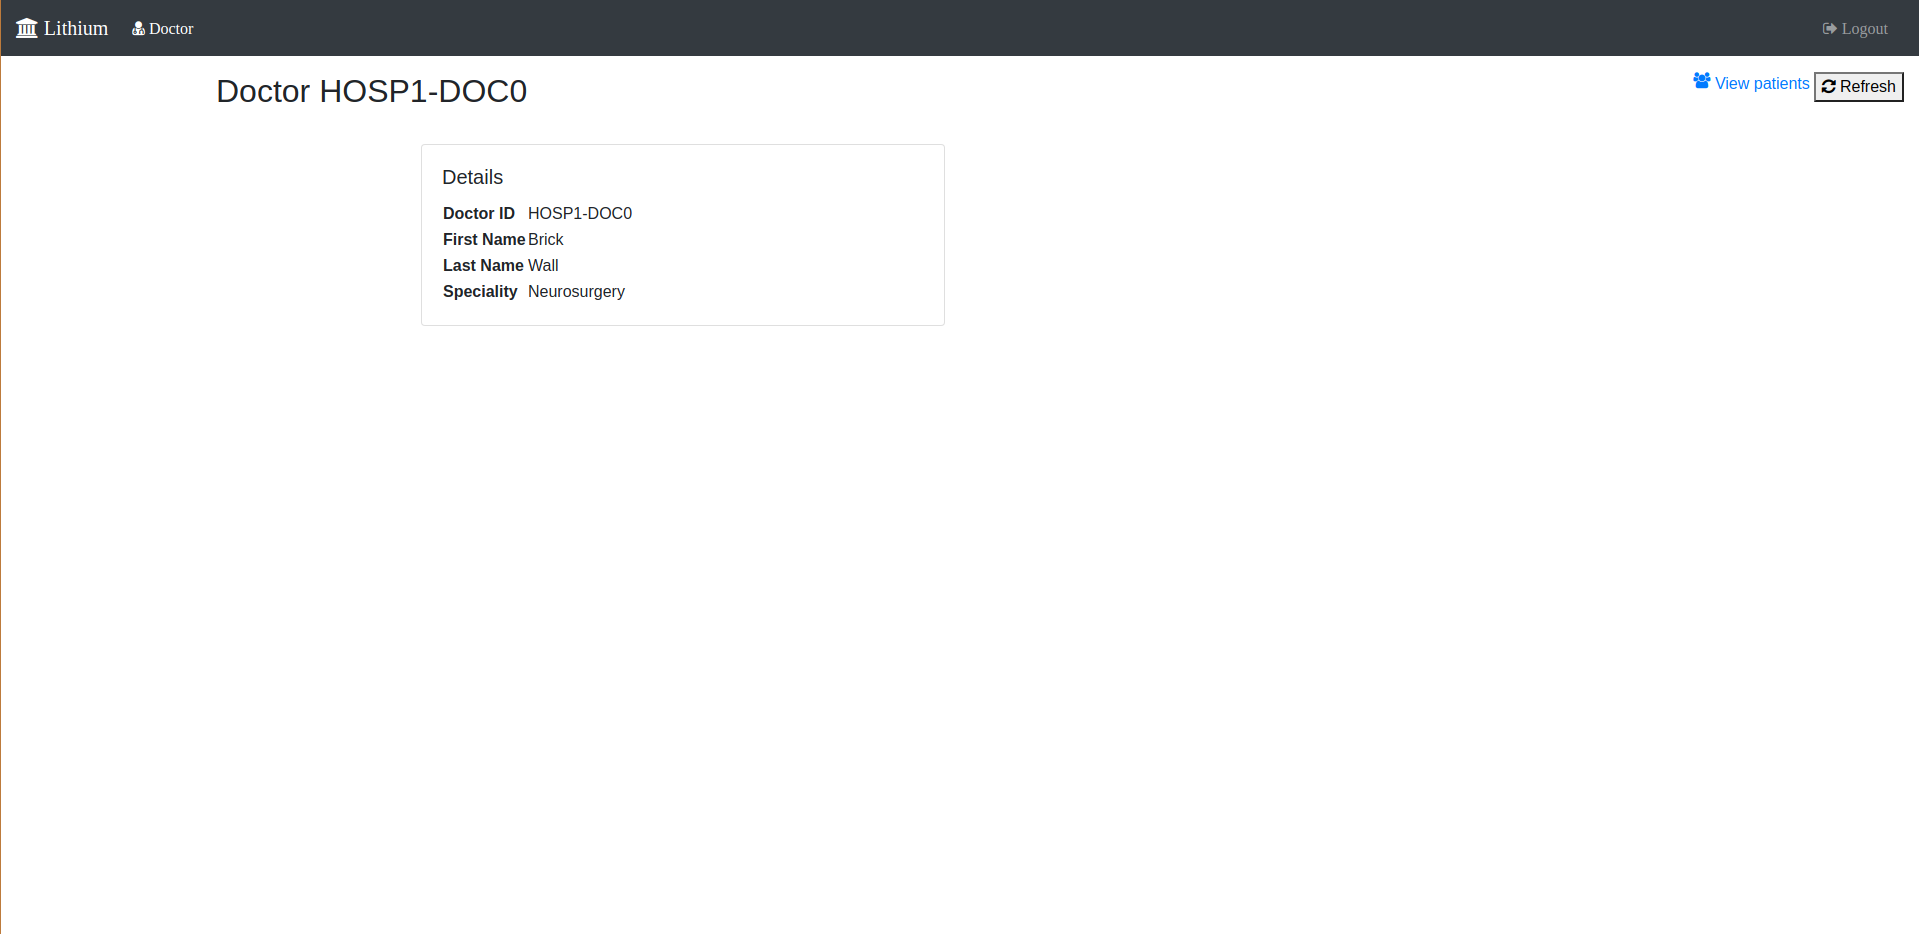
\includegraphics[width=1.1\textwidth, height=7cm]{gfx/figures/doctor2.png}
 \caption{View Doctor Details}
 \label{fig:chapter04:doctor2}
\end{figure}

\subsection{View Patients}
Doctor can view list of patients who provides access to him/her, otherwise list will be empty. In this case, the logged user doctor is 'HOSP1-DOC0' and patient PID1 provided access to this doctor. So in the list PID1 patient is visible in Figure \ref{fig:chapter04:doctor3}.

\begin{figure}[htbp]
 \centering
 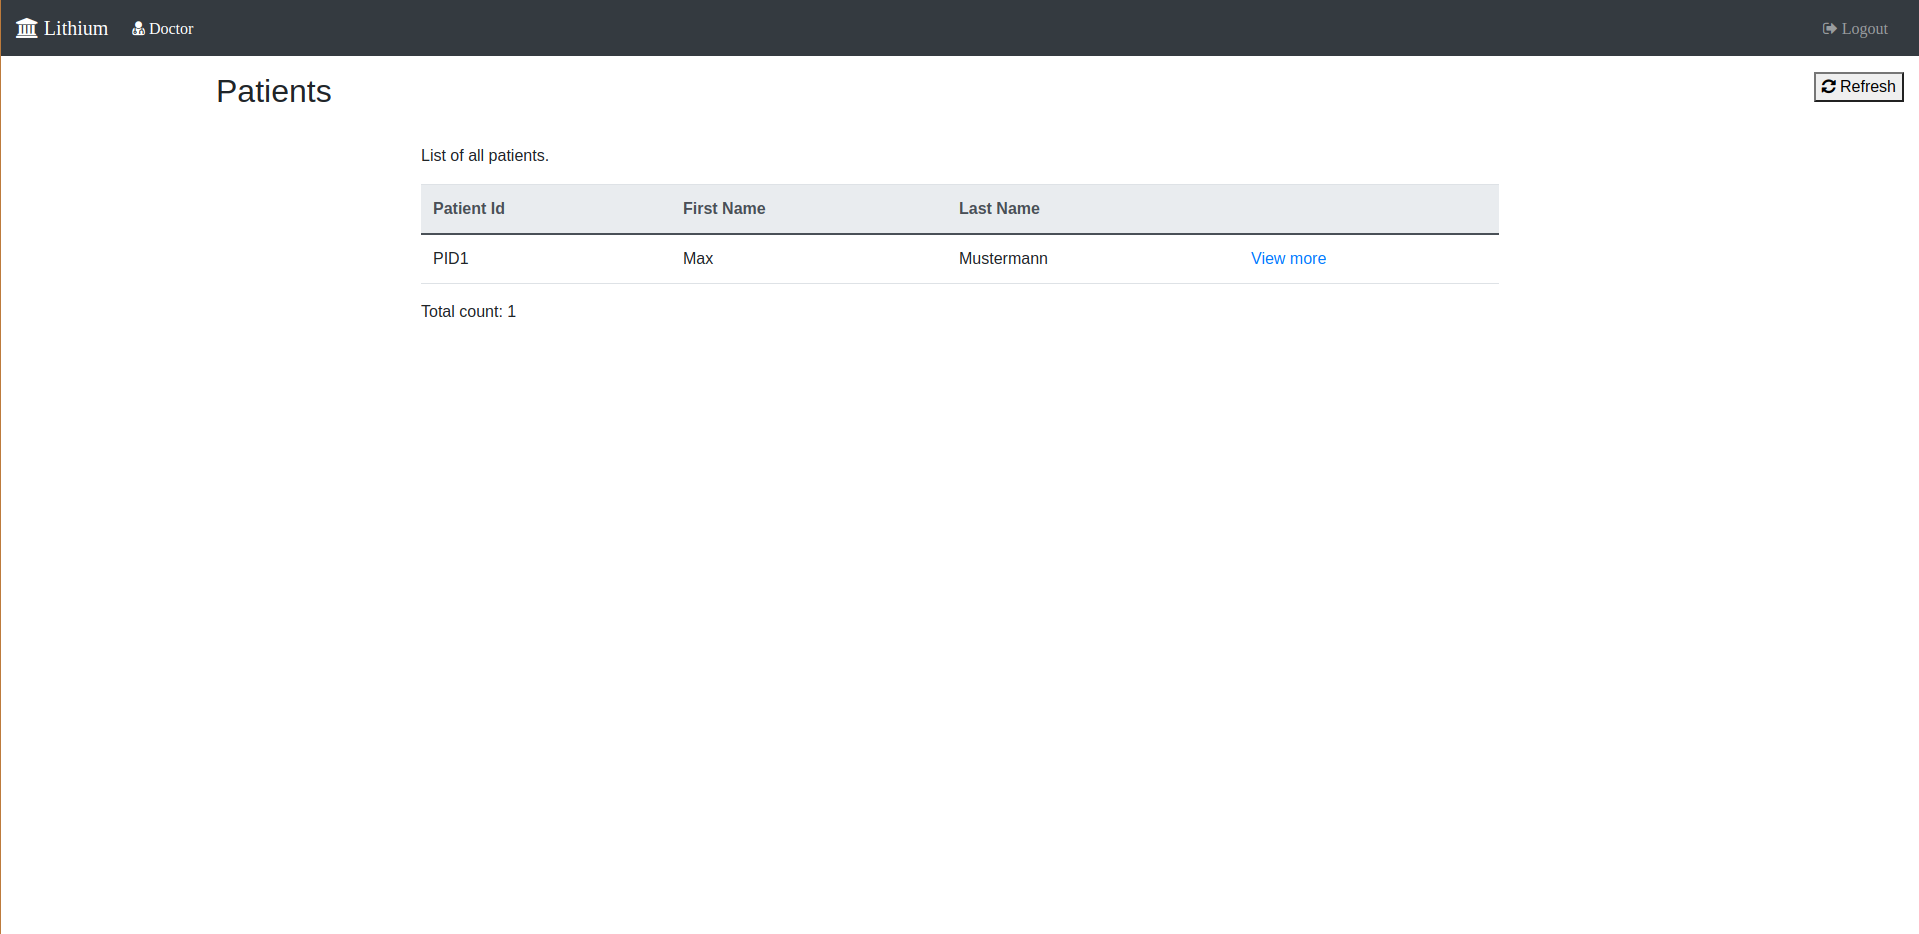
\includegraphics[width=1.1\textwidth, height=7cm]{gfx/figures/doctor3.png}
 \caption{List of patients}
 \label{fig:chapter04:doctor3}
\end{figure}

The list looks exactly same as to admin's dashboard, but doctor can see details of patient so in every entry there is a view more button as shown in Figure \ref{fig:chapter04:doctor3}. This redirects to patient details page, but only relevant fields are visible to doctor in Figure \ref{fig:chapter04:doctor4}. Here doctor can see the latest condition and information of the patient.

\begin{figure}[htbp]
 \centering
 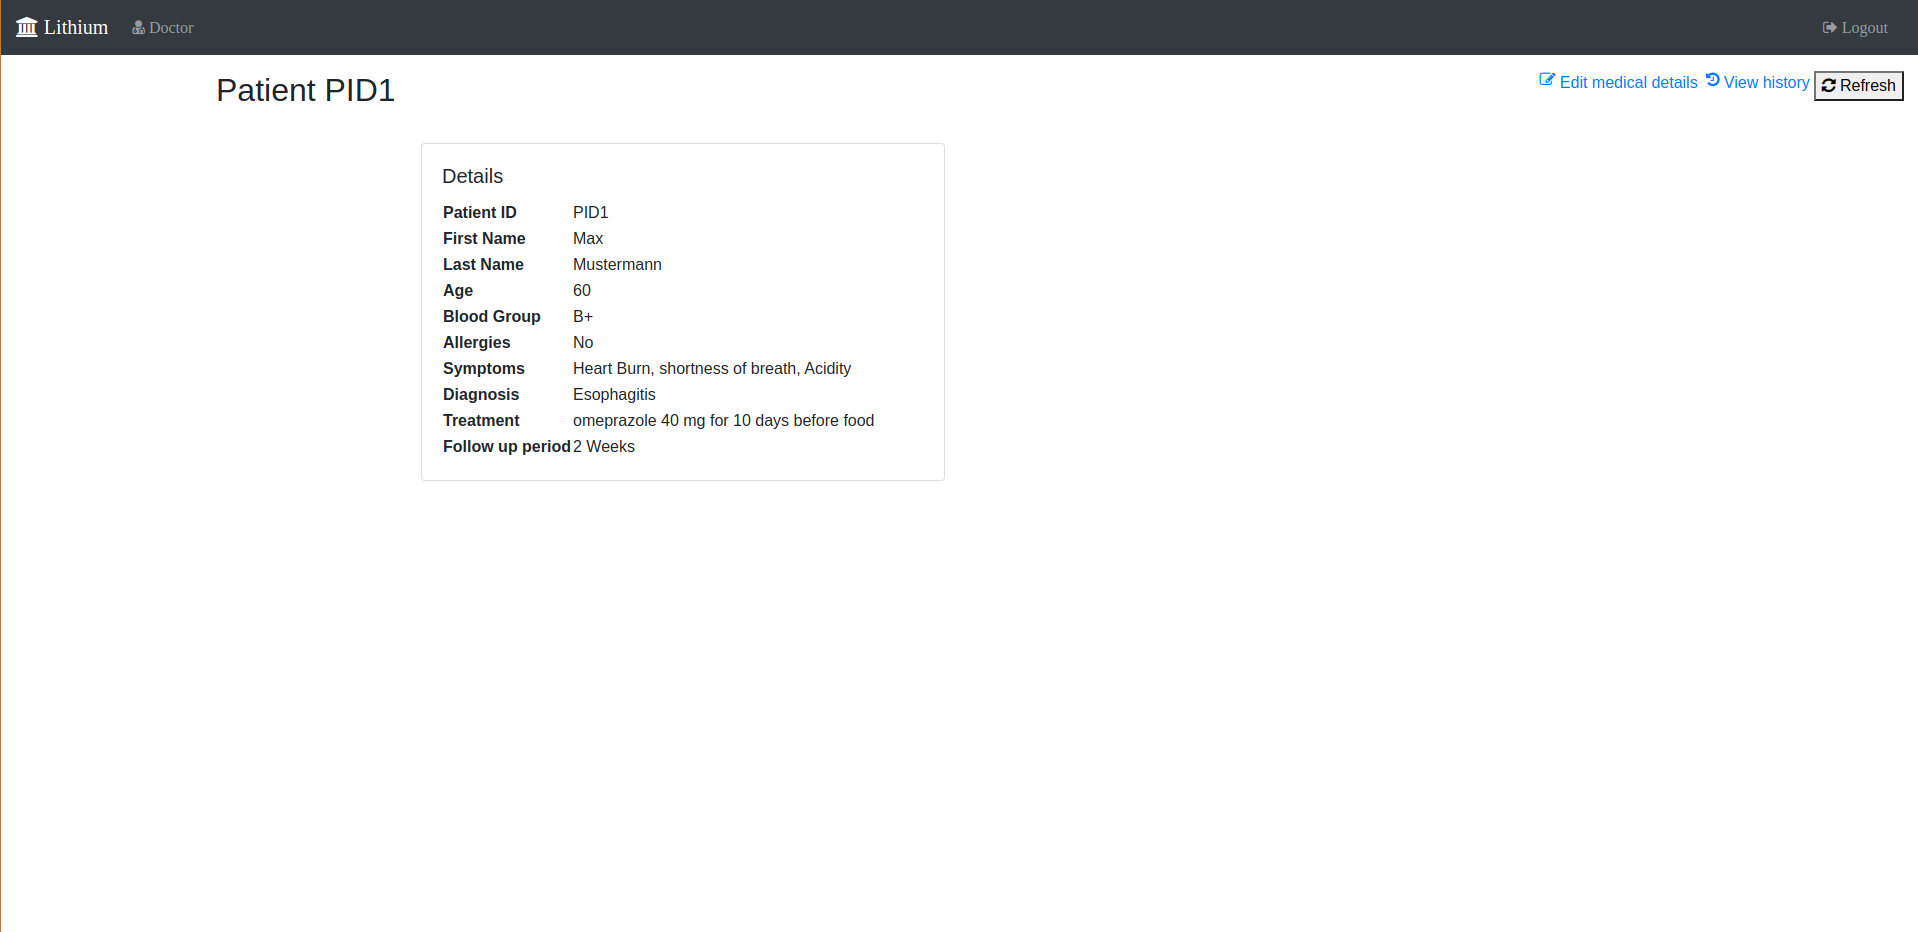
\includegraphics[width=1.1\textwidth, height=7cm]{gfx/figures/doctor4.png}
 \caption{View Patient Details}
 \label{fig:chapter04:doctor4}
\end{figure}

\subsection{Edit Medical Details}
Doctor can provide treatment by changing medical details of the patient in Figure \ref{fig:chapter04:doctor5}. On save button page redirected to patient details page.

\begin{figure}[htbp]
 \centering
 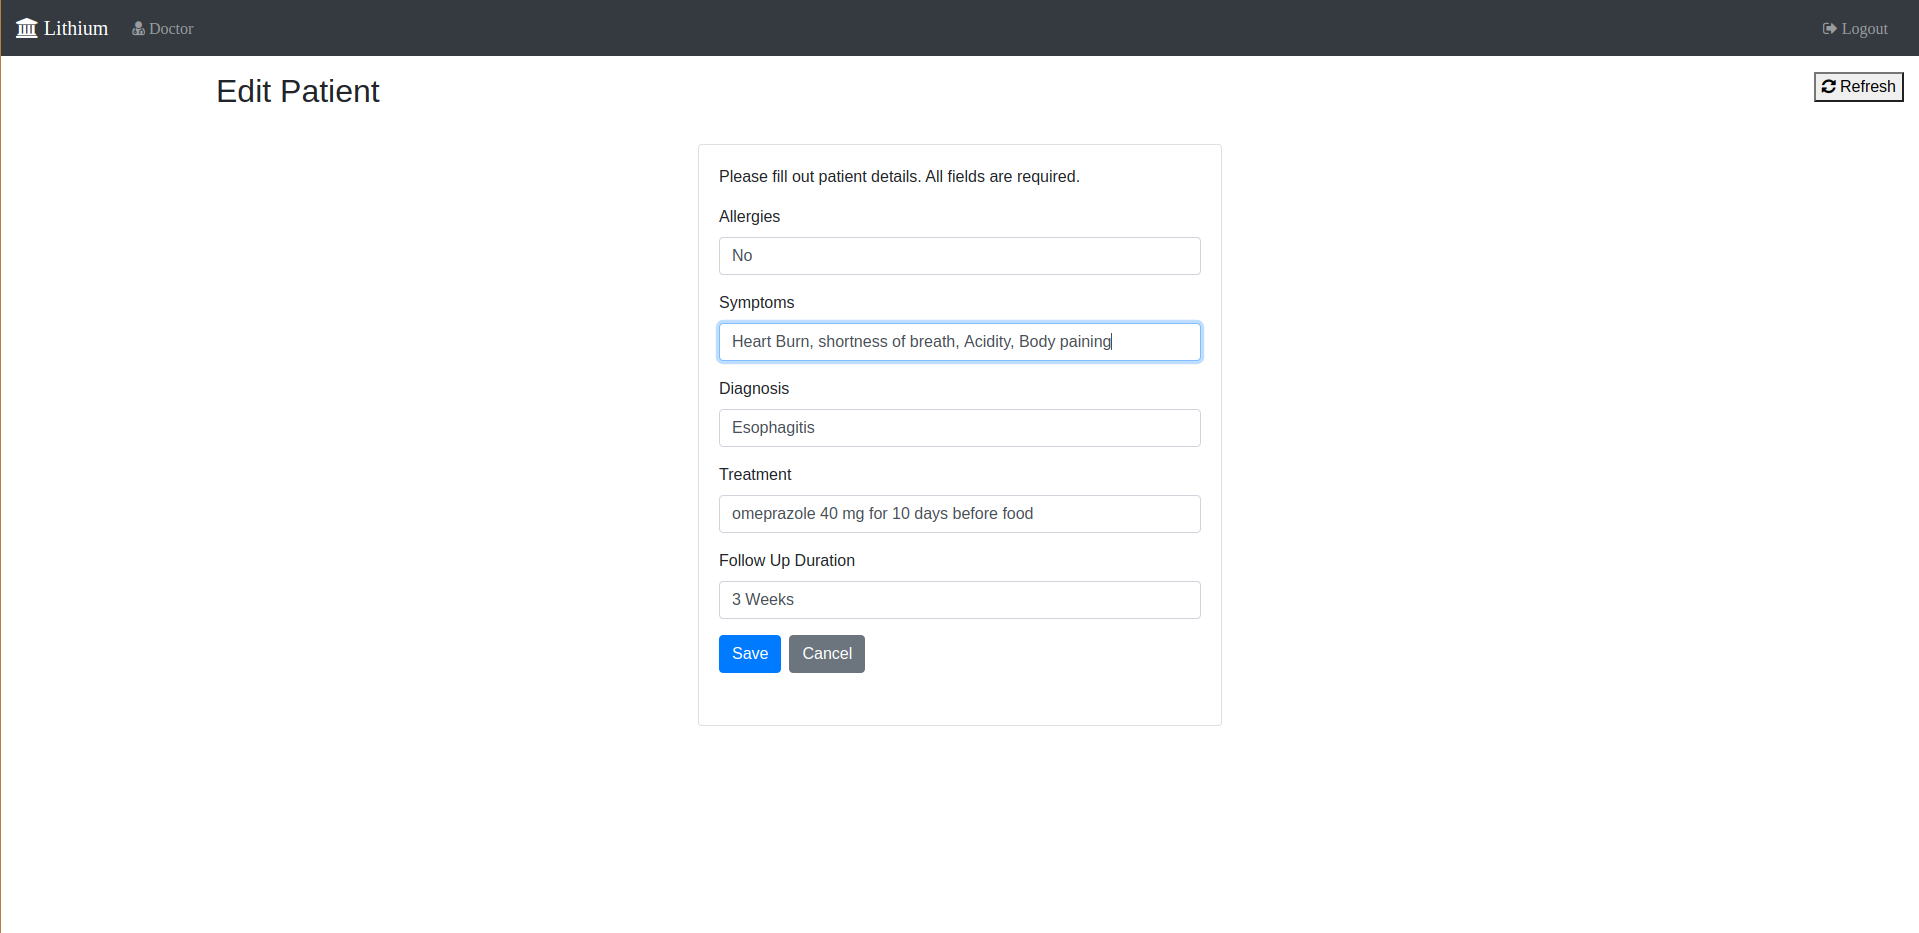
\includegraphics[width=1.1\textwidth, height=7cm]{gfx/figures/doctor5.png}
 \caption{Edit patient's medical details}
 \label{fig:chapter04:doctor5}
\end{figure}

\subsection{View History}
Doctor can view all history details of the patient which help doctor to understand patient's condition and can decide how the medication should be done. In Figure \ref{fig:chapter04:doctor6}. it shows same limited fields, as visible in patient details. In addition to those date and changed by info is also helpful to understand the treatment. 

\begin{figure}[htbp]
 \centering
 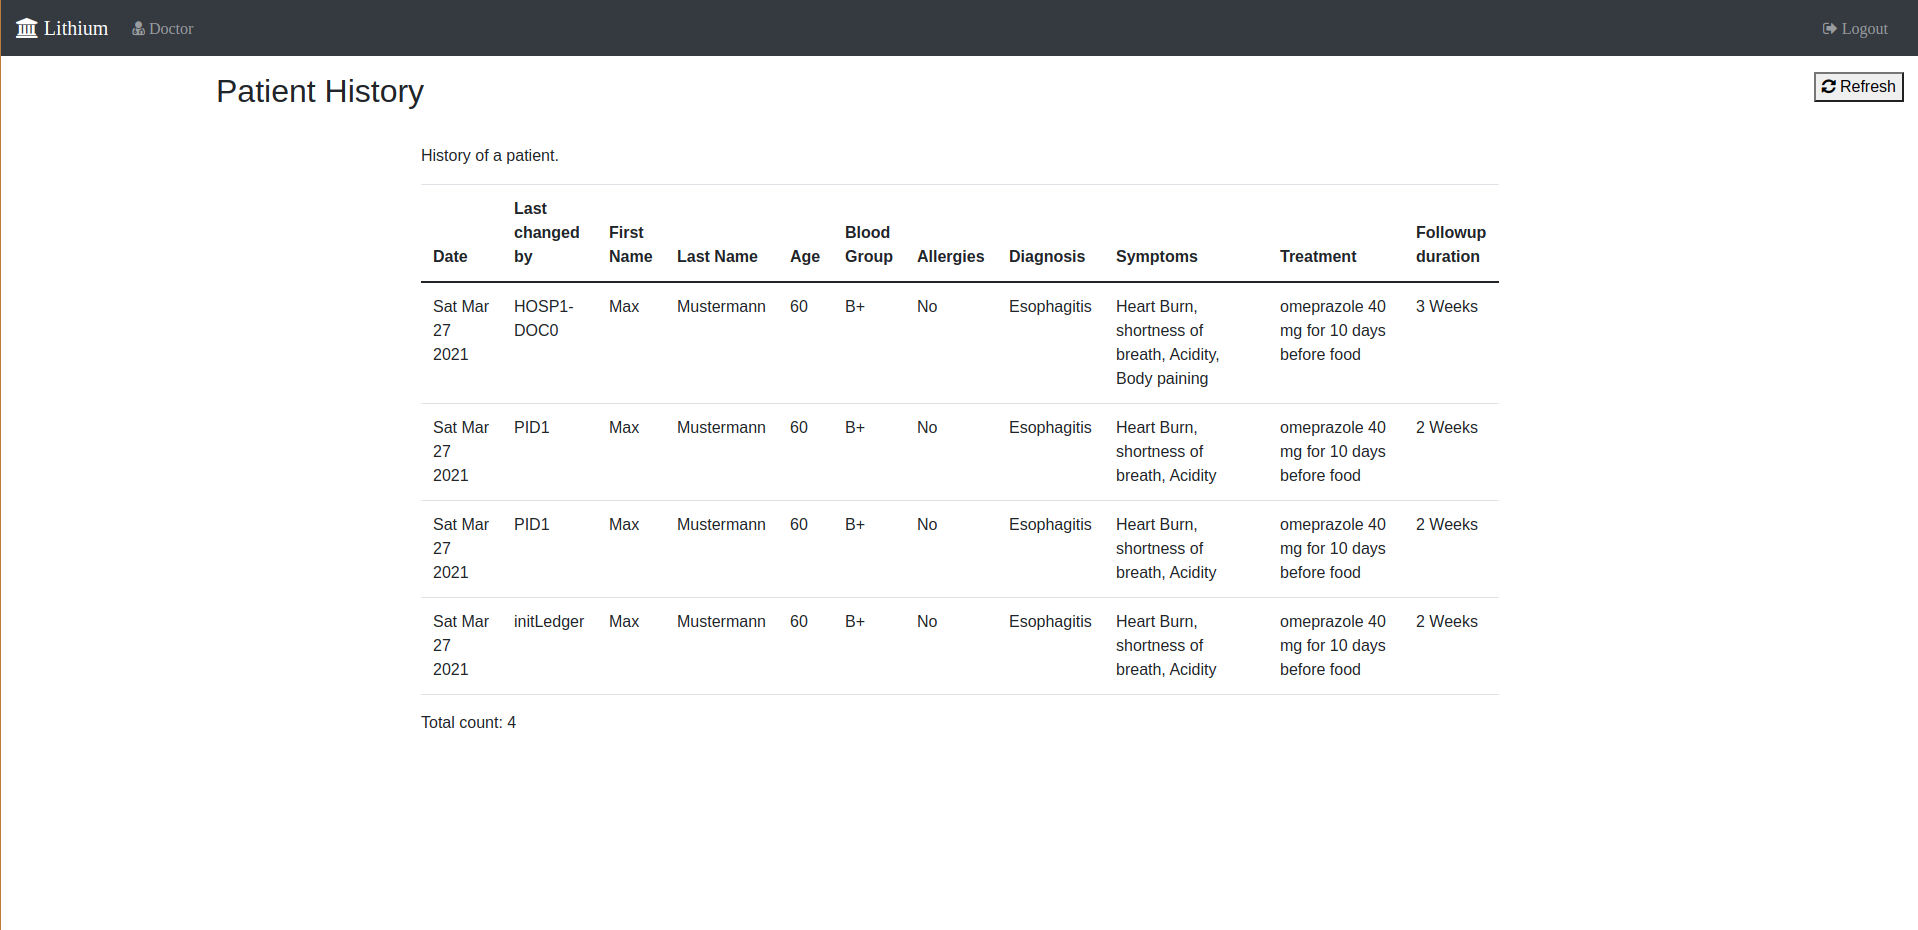
\includegraphics[width=1.1\textwidth, height=7cm]{gfx/figures/doctor6.png}
 \caption{View patient's history}
 \label{fig:chapter04:doctor6}
\end{figure}




